\section{Results}

\subsection{Medium-term direction and model-based precision}

Under the primary common two-sided 95\% Student-$t$ OLS rule, the 2010--2022 comparison yields 12 agreements, no resolved-class disagreements and 15 unresolved cases across the 27 Member States (Table~\ref{tab:mediumterm}; Figure~\ref{fig:mediumslopes}A). The released annual analysis A leaves eight directions unresolved, compared with 15 for the source-anchor analysis B1. EU27\_2020 yields one agreement, no resolved disagreement and no unresolved case under this primary rule.

Source-anchor restriction widens the classical 95\% OLS interval in every Member State (Figure~\ref{fig:mediumslopes}B). The median interval width is 0.3386 percentage points per year for A and 0.6219 for B1; the median paired B1/A width ratio is 1.858. Thus the absence of resolved directional conflict coexists with wider model-based intervals, rather than establishing equal slopes or equal precision.

The secondary common directional 95\% rule yields 15 agreements, no resolved-class disagreements and 12 unresolved Member-State comparisons. EU27\_2020 again yields one agreement and no disagreement or unresolved case. These secondary classifications use the same fits as the primary comparison.

\begin{figure}[htbp]
  \centering
  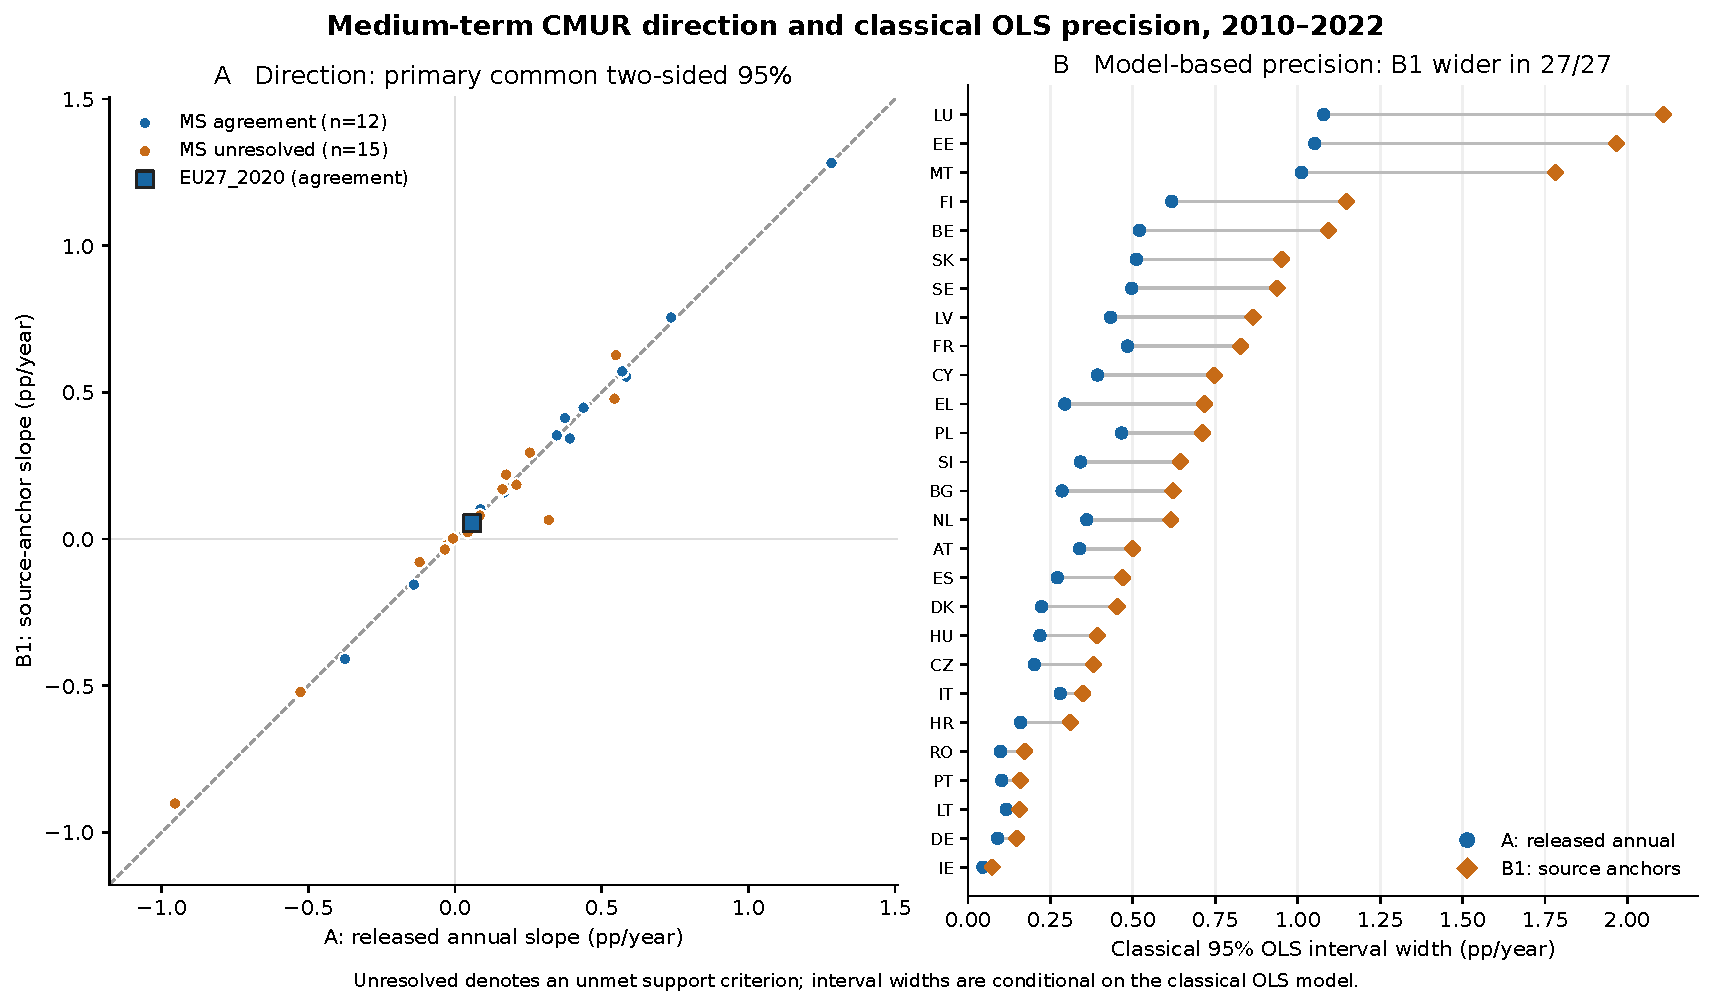
\includegraphics[width=0.82\linewidth]{figures/fig1_medium_term_slopes.pdf}
  \caption{Medium-term CMUR direction and model-based precision, 2010--2022. Panel A compares released annual A slopes with source-anchor B1 slopes. Member-State circles are grouped by the primary common two-sided 95\% comparison; the outlined square distinguishes EU27\_2020. The diagonal denotes equal slopes. Unresolved means that the primary directional support criterion is unmet in at least one series, not a resolved disagreement or evidence of no change. Panel B shows paired classical OLS 95\% interval widths for all 27 Member States, ordered by B1 width; each B1 interval is wider than its A counterpart. These widths describe precision conditional on the classical OLS model, rather than calibrated real-world uncertainty.}
  \label{fig:mediumslopes}
\end{figure}

\begin{table}[htbp]
\centering
\small
\caption{Medium-term CMUR comparison, 2010--2022: primary common two-sided 95\% and secondary common directional 95\% rules. A is the released annual series and B1 the admissible source-anchor series. Both rules use the same fixed fits. A/D/U denotes agreement/resolved-class disagreement/unresolved. Precision summaries concern Member States and classical model-based 95\% OLS intervals.}
\label{tab:mediumterm}
\begin{tabular}{llrrrrr}
\toprule
Rule & Population & A & D & U & \shortstack{A\\unresolved} & \shortstack{B1\\unresolved} \\
\midrule
\multicolumn{7}{l}{\textit{Part A: direction classification}} \\
Primary: two-sided & EU Member States & 12 & 0 & 15 & 8 & 15 \\
Primary: two-sided & EU27\_2020 & 1 & 0 & 0 & 0 & 0 \\
Secondary: directional & EU Member States & 15 & 0 & 12 & 7 & 12 \\
Secondary: directional & EU27\_2020 & 1 & 0 & 0 & 0 & 0 \\
\midrule
\multicolumn{7}{l}{\textit{Part B: Member-State classical OLS precision}} \\
\multicolumn{7}{l}{Median A interval width: 0.3386 pp/year; median B1 width: 0.6219 pp/year.} \\
\multicolumn{7}{l}{Median paired B1/A width ratio: 1.858; B1 wider: 27/27 Member States.} \\
\bottomrule
\end{tabular}
\end{table}


\subsection{Short-window support under paired residual-amplitude sensitivities}

At the reference threshold $\tau=0.95$, most through-2022 Member-State claim instances remain unresolved under both the primary unscaled empirical residual-amplitude stress scenario U and the secondary Brownian-motivated $1/\sqrt{2}$ amplitude sensitivity B (Table~\ref{tab:shortwindow}). Here A/D/U denotes agreement / resolved-class disagreement / unresolved between the released-series and source-aware classes; the final U in this triplet is a classification label, distinct from scenario U.

Annual-change comparisons yield 10/0/314 under U and 29/0/295 under B out of 324 instances. Turning yields 2/0/295 and 13/0/284, respectively, out of 297; acceleration yields 1/0/296 and 7/0/290 out of 297. There is no resolved-class disagreement at the 0.95 reference threshold in either scenario.

Relative to U, B produces 36 newly resolved Member-State comparisons: 19 annual-change, 11 turning and six acceleration instances. No final comparison loses resolution. These are outcomes of the paired residual-amplitude sensitivity, not evidence that B is closer to the unobserved true errors. For EU27\_2020, both scenarios yield 0/0/12 for annual change and 0/0/11 each for turning and acceleration at the reference threshold.

\begin{table}[htbp]
\centering
\small
\setlength{\tabcolsep}{4pt}
\caption{Source-aware short-window comparisons through 2022 at $\tau=0.95$, including the deterministic vote and minimum-three unanimity rule. U is the primary unscaled empirical stress scenario; B is the secondary Brownian-motivated $1/\sqrt{2}$ residual-amplitude sensitivity.}
\label{tab:shortwindow}
\begin{tabular}{lllrrrr}
\toprule
Population & Metric & Scenario & \shortstack{Agree-\\ment} & \shortstack{Resolved-class\\disagreement} & Unresolved & Total \\
\midrule
Member States & Annual change & U & 10 & 0 & 314 & 324 \\
Member States & Annual change & B & 29 & 0 & 295 & 324 \\
Member States & Turning & U & 2 & 0 & 295 & 297 \\
Member States & Turning & B & 13 & 0 & 284 & 297 \\
Member States & Acceleration & U & 1 & 0 & 296 & 297 \\
Member States & Acceleration & B & 7 & 0 & 290 & 297 \\
\midrule
EU27\_2020 & Annual change & U & 0 & 0 & 12 & 12 \\
EU27\_2020 & Annual change & B & 0 & 0 & 12 & 12 \\
EU27\_2020 & Turning & U & 0 & 0 & 11 & 11 \\
EU27\_2020 & Turning & B & 0 & 0 & 11 & 11 \\
EU27\_2020 & Acceleration & U & 0 & 0 & 11 & 11 \\
EU27\_2020 & Acceleration & B & 0 & 0 & 11 & 11 \\
\bottomrule
\end{tabular}
\end{table}


\subsection{Threshold robustness and the adverse resolved-disagreement case}

For every metric and both scenarios, the majority of Member-State claim instances remains unresolved at each tested threshold: 0.80, 0.85, 0.90, 0.925, 0.95, 0.975 and 0.99 (Figure~\ref{fig:shortsupport}). This persistence concerns the discrete tested values, without interpolation between them.

Resolved disagreement does occur at the lower thresholds. For BE in 2019, annual change under B is a resolved-class disagreement at $\tau=0.80$ and $0.85$: the released-series class is \textsc{negative}, whereas the source-aware class is \textsc{positive}. This comparison is unresolved at 0.90 and every higher tested threshold. The absence of disagreement at the 0.95 reference threshold therefore does not extend to the complete grid.

\begin{figure}[htbp]
  \centering
  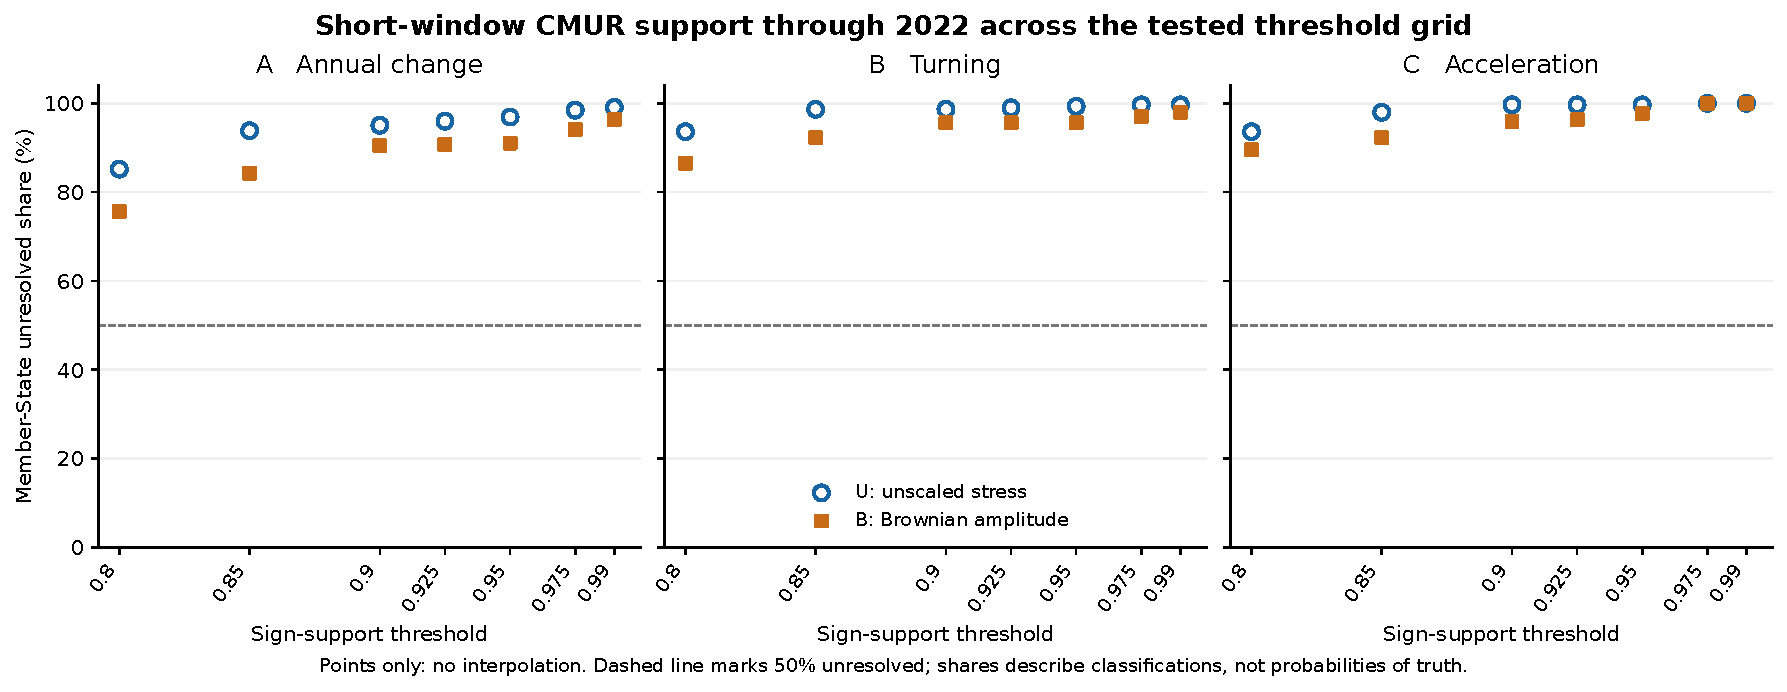
\includegraphics[width=0.80\linewidth]{figures/fig2_short_window_support.pdf}
  \caption{Member-State short-window unresolved shares through 2022 for annual change (A), turning (B) and acceleration (C). Points show the classification outcome at the seven tested sign-support thresholds for primary unscaled scenario U (hollow circles) and secondary Brownian-motivated amplitude scenario B (squares). The points are discrete evaluations, not an interpolated continuous curve. The horizontal 50\% reference marks the boundary for majority unresolvedness; both scenarios remain above it in every panel. Unresolved share records an unmet support criterion, not the probability that a claim is false or true.}
  \label{fig:shortsupport}
\end{figure}

\subsection{Supporting diagnostics and empirical boundaries}

Within the scenario-specific subsets with concordant preferred stochastic classes, Member-State median weakest-variant support changes from 0.632 under U to 0.709 under B for annual change, from 0.602 to 0.649 for turning, and from 0.557 to 0.567 for acceleration. These are descriptive conditional support summaries. The concordant subsets may differ between scenarios and are not paired subsets.

In the unscaled reference analysis, removing the deterministic midpoint vote resolves zero additional acceleration claims under either the literal minimum-three diagnostic or the separately labelled exploratory minimum-two stochastic-only diagnostic. Deterministic midpoint geometry alone is therefore insufficient to account for unresolved acceleration under this design.

The exploratory same-geography/same-centre comparison contains 76 paired cases across 26 countries, with median absolute pseudo-gap residuals of 0.525 percentage points for four-year outer spans and 0.750 for eight-year spans; the eight-year residual is larger in 54 cases, the four-year residual in 20, and two are equal, providing dependent descriptive evidence without establishing a scaling law or the true two-year error distribution.

The short-window headline comparisons end in 2022. The archived snapshot has no closing 2024 waste anchor, so source-aware endpoint claims for 2023--2024 remain unresolved under the endpoint rule and are outside these headline comparisons.
